%----------------------------------------------------------------------------------------------------
\section{Analysis}

The analysis method is similar to the previously published ones~\cite{epl101-el,prl111}, each diagonal is analysed
separately. However, a different normalisation
approach is used (Section~\ref{sec:normalisation}), making all 
$t$-independent scaling factors (e.g.~certain inefficiency corrections)
irrelevant.



%----------------------------------------------------------------------------------------------------

\subsection{Event Reconstruction}

Event kinematics are determined from track hits in the RPs after proper 
alignment (see Section~\ref{sec:alignment}), using the LHC optics 
(see Section~\ref{sec:optics}).

%------------------------------

\subsubsection{Kinematics Determination}
\label{sec:kinematics}

The horizontal ($\theta_x^*$) and vertical ($\theta_y^*$) projections of the scattering angle and the horizontal vertex position $x^*$ are first reconstructed separately from each arm, using formulae that optimise the robustness against imperfections (predominantly optics):
\begin{equation}
\label{eq:kin 1a}
	\begin{aligned}
		\theta_x^* &= {v_x^{\rm N} x^{\rm F} - v_x^{\rm F} x^{\rm N}\over v_x^{\rm N} L_x^{\rm F} - v_x^{\rm F} L_x^{\rm N}}\ ,\qquad
		\theta_y^* = {1\over 2} \left( {y^{\rm N}\over L_y^{\rm N}} + {y^{\rm F}\over L_y^{\rm F}} \right)\ ,\\
		x^* &= {L_x^{\rm N} x^{\rm F} - L_x^{\rm F} x^{\rm N}\over L_x^{\rm N} v_x^{\rm F} - L_x^{\rm F} v_x^{\rm N}}\ , \\
	\end{aligned}
\end{equation}
where the N and F superscripts refer to the near and far units, $x$ and $y$ to horizontal and vertical track hits and $v$ and $L$ stand for the magnification and effective length optical functions. This one-arm reconstruction is used for tagging elastic events, where the left and right arm protons are compared. Once an event is selected, the information from both arms can be merged yielding better angular resolution:
\begin{equation}
\label{eq:kin 2a}
\theta_x^* = {\theta_x^{*\rm L} + \theta_x^{*\rm R} \over 2}\ ,\quad \theta_y^* = {\theta_y^{*\rm L} + \theta_y^{*\rm R} \over 2}\ ,
\end{equation}
where the L (R) superscript refers to the left (right) arm.

Eventually, the full scattering angle, $\theta^*$, and four-momentum transfer squared, $t$, are calculated as

\begin{equation}
\label{eq:th t}
\theta^* = \sqrt{{\theta_x^*}^2 + {\theta_y^*}^2}\ ,\quad t = - p^2 ({\theta_x^*}^2 + {\theta_y^*}^2)\ ,
\end{equation}
where $p$ denotes the beam momentum.

%------------------------------

\subsubsection{Alignment}
\label{sec:alignment}

The standard three-step procedure \cite{totem-ijmp} has been applied: beam-based alignment prior to the run (as for LHC collimators) followed by two off-line methods: track-based alignment (for relative positions among RPs) and alignment with elastic events (for absolute position with respect to the beam). The final uncertainties per unit (common for top and bottom RPs) are: $2\un{\mu m}$ (horizontal shift), $100\un{\mu m}$ (vertical shift) and $0.2\un{mrad}$ (rotation about the beam axis). Propagated to the scattering angles, Eq.~(\ref{eq:kin 2a}), the shifts lead to uncertainties of $0.8\un{\mu rad}$ (horizontal) and $0.2\un{\mu rad}$ (vertical). The error of the RP rotations would bias the reconstructed $\theta_x^*$ by a term proportional to $\theta_y^*$, with the proportionality constant having a standard deviation of $0.02$.


%------------------------------

\subsubsection{Optics}
\label{sec:optics}

In order to reduce the impact of imperfect optics knowledge, the optics matching technique \cite{totem-optics} has been applied. The residual imperfections induce an error in the reconstructed scattering angle proportional to the angle. For the two-arm reconstruction, Eq.~(\ref{eq:kin 2a}), the proportionality constants have uncertainties of $0.21\un{\%}$ (horizontal) and $0.25\un{\%}$ (vertical), including the effects of magnet harmonics.

\iffalse
% original text
In order to reduce errors due to imperfect optics knowledge, the optics matching technique \cite{totem-optics} has been applied. The 
corrections have the form of factors scaling the scattering angles
For the two-arm reconstruction, Eq.~(\ref{eq:kin 2a}), the factors have uncertainties of $0.21\un{\%}$ (horizontal) and $0.25\un{\%}$ (vertical), including the effects of magnet harmonics.
\fi

% double-arm; before matching $0.48\un{\%}$ (hor), $0.90\un{\%}$


%------------------------------

\subsubsection{Resolution}
\label{sec:resolution}

Statistical fluctuations in the reconstructed scattering angles are caused by 
the beam divergence and, in the horizontal projection (due to small $L_x$), 
also by the sensor resolution (strip pitch). Good descriptions of these effects
are essential for several corrections discussed below.

The angular resolution is studied through differences $\theta_{x,y}^{*R} - \theta_{x,y}^{*L}$. Since in good approximation the fluctuations are independent in each arm, the distribution of the difference is just twice wider than the fluctuation of angles in Eq.~(\ref{eq:kin 2a}). Generally, the distributions are well Gaussian, the small non-Gaussianity is decreasing with time. The resolutions were found to deteriorate with time: for the two-arm $\theta_y^*$ it evolved from initially $1.6$ to $1.7\un{\mu rad}$ at the end of the run. For $\theta_x^*$, the resolution decreased from $4.6$ to $4.8\un{\mu rad}$ (for the diagonal 45 bottom -- 56 top) and from $4.3$ to $4.4$ (45 top -- 56 bottom).

Measurements of beam emittances show that the vertical beam divergences of the two beams are equal with a tolerance of about $15\un{\%}$. Exploiting this equality, one can de-convolute the distribution of $\theta_y^{*R} - \theta_y^{*L}$ in order to obtain the beam-divergence distribution, used e.g.~for acceptance corrections (see Section~\ref{sec:acc corr}).


\iffalse
The resolution in $\theta_y^*$ decreased from $1.6$ to $1.7\un{\mu rad}$ from the beginning to the end of the fill (DS3+DS4), for $\theta_x^*$ from $4.6$ to $4.8\un{\mu rad}$ (45b -- 56t) and from $4.3$ to $4.4\un{\mu rad}$ (45t -- 56b). In fact, just means over all bunches -- in analysis bunches treated independently. Comparing x and y, the contribution from the RP spatial resolution is evident. A cross check, horizontal beam div. from vertex distribution (sigma 145 to 185 urad, diagonal independent) % 2.3 to 2.9 urad
, the sensor contribution (2-arm) is $4.3$ (45b) and $4.0$ urad (45t), time independent. With the same method, not only RMS, but also shape. Generally, gaussian-like, with non-gaussianity decreasing with time. Non-gaussianinty taken accounted in systematic uncertainties. The original assumption of identical resolutions in both arms can be verified by checking the beam emittances. They give beam divergences compatible with our observations and indicate that a possible left-right imbalance could be of order $15\un{\%}$, which is used for uncertainty estimation.
\fi

%----------------------------------------------------------------------------------------------------

\subsection{Differential Cross-Section}
\label{sec:diff cs}

For a given $t$ bin, the differential cross-section is evaluated by selecting and counting elastic events:
\begin{equation}
{\d\sigma\over \d t}(\hbox{bin}) =
	{\cal N}\, {\cal U}({\rm bin})\, {\cal B}\ 
	{\sum\limits_{t \in \hbox{bin}} {\cal A}(\theta^*, \theta_y^*)\, {\cal E}(\theta_y^*)\over \Delta t}\ ,
\end{equation}
where $\Delta t$ is the width of the bin, ${\cal N}$ is a normalisation factor, 
and the other symbols stand for various correction factors:
${\cal U}$ for unfolding of resolution effects, ${\cal B}$ for background subtraction, ${\cal A}$ for acceptance correction and ${\cal E}$ for detection and reconstruction efficiency.

%------------------------------

\subsubsection{Event Tagging}
\label{sec:tagging}

The cuts used to select elastic events are summarised in Table \ref{tab:cuts}, all are applied at the $4\sigma$ level. Cuts 1 and 2 require the reconstructed-track collinearity between the left and right arm. Cuts 3 and 4 control the elasticity -- if a proton loses momentum, the vertical position-angle correlation at the RPs is lost. Cut 5 ensures that the two protons come from the same vertex (horizontally). 

The tagging efficiency is studied by applying the cuts also at the $5\un{\sigma}$ level. This selection yields about $0.5\un{\%}$ more events in every $t$ bin -- thus the inefficiency is irrelevant for the presented analysis.

\begin{table}
\caption{The elastic selection cuts. The superscripts R and L refer to the right and left arm, N and F correspond to the near and far units, respectively. The constant $\alpha = L_y^{\rm F} / L_y^{\rm N} - 1 \approx 0.107$. The right-most column gives a typical RMS of the cut distribution.
}
\label{tab:cuts}
\begin{center}
\vskip-3mm
\begin{tabular}{ccc}\hline\hline
number & cut & RMS ($\equiv 1\sigma$)\cr\hline
1 & $\theta_x^{*\rm R} - \theta_x^{*\rm L}$				& $9.5\un{\mu rad}$	\cr
2 & $\theta_y^{*\rm R} - \theta_y^{*\rm L}$				& $3.3\un{\mu rad}$	\cr
3 & $\alpha\,y^{\rm R,N} - (y^{\rm R,F} - y^{\rm R,N})$	& $18\un{\mu m}$	\cr
4 & $\alpha\,y^{\rm L,N} - (y^{\rm L,F} - y^{\rm L,N})$	& $18\un{\mu m}$	\cr
5 & $x^{*\rm R} - x^{*\rm L}$							& $8.5\un{\mu m}$ 	\cr\hline\hline
\end{tabular}
\end{center}
\end{table}

%------------------------------

\subsubsection{Background}
\label{sec:background}

Studying distributions of discriminators from Table~\ref{tab:cuts} under various cut combinations allows for separation of signal and background contributions. While the central part (signal, within $4\un{\sigma}$) remains essentially constant, the tails (background) are dramatically affected. Interpolating the background smoothly into the signal region yields a background estimate of $1 - {\cal B} < 10^{-4}$ (independent of whether discriminator 1, 2 or 5 is used).
% anyway irrelevant due to the normalisation approach

%-------------------------

\subsubsection{Acceptance Correction}
\label{sec:acc corr}

Two detection limitations have been identified: detector coverage (mostly at the edge facing the beam, i.e. relevant for small $|\theta_y^*|$) and LHC apertures ($|\theta_y^*| \sim 100\un{\mu rad}$). The acceptance correction includes two contributions -- a geometrical correction ${\cal A}_{\rm geom}$ reflecting the fraction of the phase space within the acceptance and a component ${\cal A}_{\rm fluct}$ correcting for fluctuations around the acceptance limitations:
\begin{equation}
{\cal A}(\theta^*, \theta_y^*) = {\cal A}_{\rm geom}(\theta^*)\ {\cal A}_{\rm fluct}(\theta_y^*)\ .
\end{equation}

The calculation of the geometrical correction ${\cal A}_{\rm geom}$ is based on the azimuthal symmetry of elastic scattering, experimentally verified for the data within acceptance. The correction is given by the inverse of the fraction of a circle with radius $\theta^*$ falling into the acceptance region in the ($\theta_x^*$, $\theta_y^*$) space. The value of the correction drops rapidly from $5$ at the lowest $|t|$ to about $2.5$ at $|t| = 0.15\un{GeV^2}$ and then increases again to about $4$ at $|t| = 0.2\un{GeV^2}$.

The correction ${\cal A}_{\rm fluct}$ is calculated analytically from the probability that any of the two elastic protons is pushed outside the acceptance due to the beam divergence. The beam divergence distribution is modelled as Gaussian with spread determined by the method described in Section~\ref{sec:resolution}. This correction contribution is only sizeable close to the acceptance limitations but remains below $1.5$. The uncertainties are related to the resolution parameters (vertical beam divergence, left-right asymmetry and non-Gaussian shape), and all stay below $0.1\un{\%}$.


\iffalse
\begin{equation}
\label{acceptance}
{\cal A_{\rm sm}}(\theta_y^*)^{-1} = {1\over 2} \left(
	\mathop{\rm Erf} {\min(\theta_y^{*,R,max} - |\theta_y^*|, |\theta_y^*| - \theta_y^{*,L,min})\over \sigma^{1a}_{\theta_y^*}}
	- \mathop{\rm Erf} {\max(\theta_y^{*,R,min} - |\theta_y^*|, |\theta_y^*| - \theta_y^{*,L,max})\over \sigma^{1a}_{\theta_y^*}}
\right)
\end{equation}

\begin{equation}
\label{acceptance}
{\cal A_{\phi}}(\theta_y^*) = {
	2\pi\over 
	\hbox{arc length with $\theta_y^*$ between } \max(\theta_y^{*,L,min}, \theta_y^{*,R,min}) \hbox{ and } \min(\theta_y^{*,L,max}, \theta_y^{*,R,max})
}
\end{equation}
\fi

%-------------------------

\subsubsection{Inefficiency Corrections}
\label{sec:ineff corr}

Any inefficiency correction that does not alter the $t$-distribution shape does not need to be considered in this analysis (e.g.~the pile-up inefficiency discussed in \cite{prl111}).

The uncorrelated 1-RP inefficiency ${\cal I}_{3/4}$ is evaluated by removing a given RP from the tagging cuts, Table \ref{tab:cuts}, and calculating the fraction of recovered events. This fraction has been found to depend gently on the vertical scattering angle. The average slope of the decrease per RP is $80\un{rad^{-1}}$ with a typical uncertainty of $8\un{rad^{-1}}$.

The 1-RP inefficiencies are complemented by near-far correlated inefficiencies ${\cal I}_{2/4}$ from proton interactions in the near RP affecting also the far one. This contribution is determined by counting events with corresponding shower signatures and is validated with a Monte-Carlo simulation.

The full correction is calculated as
\begin{equation}
\label{efficiency}
	{\cal E}(\theta_y^*) = {1\over 1 - \left( \sum\limits_{i\in \rm RPs} {\cal I}^i_{3/4}(\theta_y^*) + 2 {\cal I}_{2/4} \right) } \ ,
\end{equation}
where the first term in parentheses typically grows from about $7$ to $10\un{\%}$ from the lowest to the highest $|\theta_y^*|$ and the second term amounts to about $3\un{\%}$.

%Trigger efficiency. Zero-bias data stream, events tagged as elastic, look at the trigger flag. NOT IN DS4 !!!
%For example for DS2, at $95\un{\%}$ CL, ${\cal I}_{\rm trig} < 8\cdot10^{-4}$. Anyway irrelevant.


%-------------------------

\subsubsection{Unfolding of Resolution Effects}
\label{sec:unfolding}

The correction for resolution effects has been determined by the following iterative procedure. The differential cross-section data are fitted by a smooth curve which serves as an input to a Monte-Carlo simulation using the resolution parameters determined in Section~\ref{sec:resolution}. Making a ratio between simulated histograms with and without smearing effects gives a set of per-bin correction factors. Applying them to the yet uncorrected differential cross-section yields a better estimate of the true $t$-distribution which can be used as input to the next iteration. Due to the relatively good angular resolution, the final correction is not large: $|1 - {\cal U}| < 3\un{\%}$.

For the uncertainty estimate, the uncertainties of $\theta_x^*$ and $\theta_y^*$ resolutions (accommodating the full time variation) as well as fit-model dependence have been considered, the first contribution being dominant.

%2 iterations


%-------------------------

\subsubsection{Normalisation}
\label{sec:normalisation}

The normalisation ${\cal N}$ is determined by requiring the same cross-section integral between $|t| = 0.027$ and $0.083\un{GeV^2}$ as for dataset 1 from \cite{prl111}, where the luminosity-independent calibration was applied. The leading uncertainty of the scaling factor $4.2\un{\%}$ comes from the luminosity-independent %\linebreak 
method.

%Leading uncertainty: lumi error from DS2 ($4.2\un{\%}$), transfer to DS4 negligible (few per-mille)


%-------------------------

\subsubsection{Binning}
\label{sec:binning}

Two binnings have been considered. The ``optimised'' option sets the bin size to $1\un{\sigma}$ of the resolution in $t$. The ``per-mille'' binning is built such that each bin collects about one per-mille of the events.


%-------------------------

\subsubsection{Systematic Uncertainties}
\label{sec:systematics}

Besides the systematic uncertainties mentioned at the above analysis steps, the uncertainty of the beam momentum, $0.1\un{\%}$, needs to be considered when the scattering angles are translated into $t$, see Eq.~(\ref{eq:th t}). The systematic effects are propagated to the $t$-distribution by inserting the final cross-section into a Monte-Carlo simulation where any analysis parameter can be artificially biased.
%The results are validated with a semi-analytical calculation eventually exploiting numerical integration.



%----------------------------------------------------------------------------------------------------

\subsection{Systematic Cross-Checks}
\label{sec:cross checks}

Compatible results have obtained from data originating from different bunches and different diagonals and different time periods.

%----------------------------------------------------------------------------------------------------

\subsection{Final Data Merging}
\label{sec:final data merging}

Eventually, the differential cross-section histograms from both diagonals are merged. This is accomplished by a per-bin weighted average, with the weight given by inverse squared statistical uncertainty. The statistical and systematic uncertainties are propagated accordingly. For the systematic ones, the correlation between the diagonals is taken into account. For example the vertical (mis-)alignment of the RPs within one unit is almost fully correlated, thus the effect on the differential cross-section is opposite in the two diagonals, and consequently its impact is strongly reduced once the diagonals are merged.

The systematic uncertainties are summarised in Figure~\ref{fig:syst unc} where their impact on the differential cross-section is shown. The leading uncertainties include normalisation, optics imperfections and beam momentum offset. They are quantified in Table~\ref{tab:data} and can be used to approximate the covariance matrix of systematic uncertainties:
\begin{equation}
\label{eq:covar mat}
\mat V = \sum_{i} \vec v_i \vec v_i^{\rm T}\ ,
\end{equation}
where the $\vec v_i$'s represent the uncertainty vectors (columns) from the table.

\begin{figure*}[t]
\begin{center}
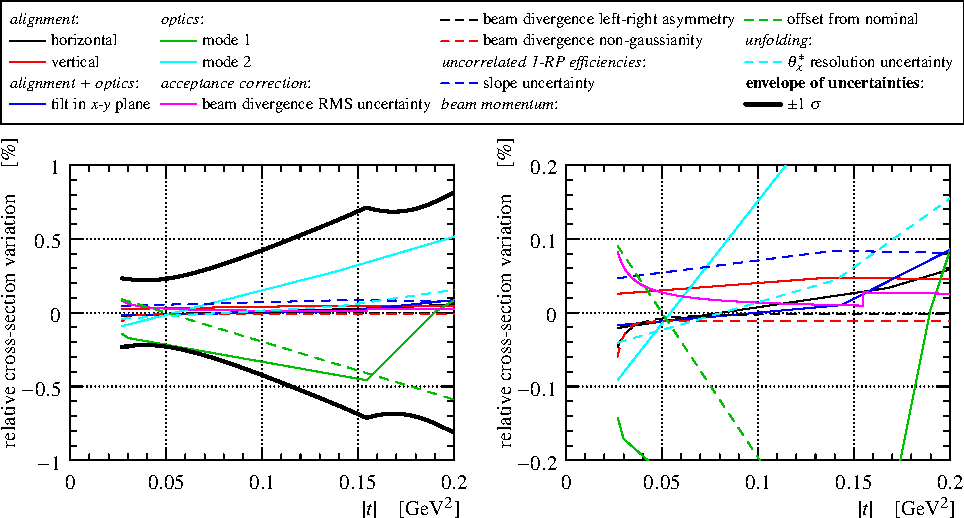
\includegraphics[width=13cm]{fig/direct_method_mode_cmp_presentation.pdf}
\caption{%
Impact of systematic uncertainties on the differential cross-section. The two contributions due to optics correspond to the two eigenvectors of the covariance matrix of the factors scaling $\theta_x^*$ and $\theta_y^*$ (see Section~\ref{sec:optics}).
}
\label{fig:syst unc}
\end{center}
\end{figure*}

%----------------------------------------------------------------------------------------------------

\subsection{Statistical Uncertainty Adjustment}
\label{sec:stat unc adj}
%
Examining point-to-point fluctuations in the differential cross-section using the optimised binning indicates that the statistical fluctuations have been slightly overestimated. This can be alternatively demonstrated by the following procedure. The data sample is divided into several sub-samples corresponding to the same luminosity and the above-described analysis method is repeated for all of them. Then fluctuations of each bin content are determined from the several sub-samples, giving values slightly lower than the uncertainty estimates. A similar problem does not occur for the per-mille binning.
%\todo{Interpretation?}.
As a remedy, the statistical uncertainties in the optimised binning have been divided by factor $1.176$ determined by requiring the same $\chi^2$ as for the per-mille binning when a function with enough degrees of freedom is used (see the green fit in Figure~\ref{fig:data rel ob}).


%----------------------------------------------------------------------------------------------------
\section{Results}

% --- the results drawn from the optimised binning

The final differential cross-section in the optimised binning is presented in Table~\ref{tab:data}. Since it exhibits an exponential-like fall-off, for visualisation purposes, it is preferable to plot the relative difference of the cross-section from a reference exponential, % subtracting the main component
see Figure~\ref{fig:data rel ob}. This plot immediately suggests a non-exponentiality of the data. To quantify this observation, a series of fits has been made using this parametrisation:
\begin{equation}
\label{fit param}
{\d\sigma\over\d t}(t) = \left. \d\sigma\over\d t\right|_{0} \ \exp\left( \sum\limits_{i = 1}^{N_{b}} b_i\, t^i \right) \:.
\end{equation}
The fits have been performed by minimising the standard $\chi^2$ with the covariance matrix given by the sum of the statistical and systematic components. The fit results are shown in Figure~\ref{fig:data rel ob}, clearly indicating that the purely-exponential fit ($N_b = 1$) is excluded at $7.2\un{\sigma}$ significance. The other two fits present very reasonable p-values and can, therefore, be used for a total cross-section estimation with the optical theorem in the form
\begin{equation}
\label{eq:si tot}
\sigma_{\rm tot}^2 = {16\pi\, (\hbar c)^2\over 1 + \rho^2}\, \left. \d\sigma_{\rm el}\over\d t\right|_0\ ,
\end{equation}
for the first time using a non-exponential extrapolation to $t=0$. Using the COMPETE~\cite{compete} preferred-model extrapolation of $\rho = 0.140\pm 0.007$ yields
\begin{equation}
\label{eq:si tot results}
	\begin{aligned}
		N_b &= 2:\quad \sigma_{\rm tot} = (100.8 \pm 2.1)\un{mb}\ ,\\	% A = 529.3 +- 21.9
		N_b &= 3:\quad \sigma_{\rm tot} = (101.2 \pm 2.1)\un{mb}\ ,\\	% A = 533.5 +- 21.9
	\end{aligned}
\end{equation}
which are well compatible with the previous measurement using the luminosity-independent method~\cite{prl111}.




\begin{table*}[t!]
\caption{%
The elastic differential cross-section as determined in this analysis using the optimised binning. The three left-most columns describe the bins in $t$. The representative point gives the $t$ value suitable for fitting~\cite{lafferty94}. %uncertainty due to different fit models negligible:$10^{-7}\un{GeV^2}$
The other columns are related to the differential cross-section. The four right-most columns give the leading systematic uncertainty modes (see Section~\ref{sec:final data merging} and Figure~\ref{fig:syst unc}).
}
\label{tab:data}
\begin{center}
\small
\setlength{\tabcolsep}{3.5pt}
\begin{tabular}{ccc@{\hskip20pt}ccccccc}
\hline
\hline
\multispan3\hss\vrule width0pt depth4pt height10pt $|t|$ bin $\unt{GeV^2}$\hss & \multispan7\hss $\d\sigma/\d t \ung{mb/GeV^2}$ \hss \cr
\multispan3\hrulefill\hbox to15pt{\hfil} & \multispan7\hrulefill \cr
left & right & representative & value & statistical     & systematic  & normalisation & optics   & optics   & beam\cr
edge & edge  & point      &       & uncertainty      & uncertainty   &       & mode 1   & mode 2   & momentum\cr
\hline
$0.02697$ & $0.03005$ & $0.02850$ & $300.94\S$ & $0.612\S$ & $12.68\S$ & $+12.66\S$ & $-0.473\S$ & $-0.259\S$ & $+0.254\S$ \cr
$0.03005$ & $0.03325$ & $0.03164$ & $284.04\S$ & $0.554\S$ & $11.91\S$ & $+11.90\S$ & $-0.495\S$ & $-0.214\S$ & $+0.204\S$ \cr
$0.03325$ & $0.03658$ & $0.03491$ & $265.59\S$ & $0.506\S$ & $11.17\S$ & $+11.15\S$ & $-0.484\S$ & $-0.172\S$ & $+0.157\S$ \cr
$0.03658$ & $0.04005$ & $0.03831$ & $247.90\S$ & $0.465\S$ & $10.44\S$ & $+10.43\S$ & $-0.472\S$ & $-0.133\S$ & $+0.114\S$ \cr
$0.04005$ & $0.04365$ & $0.04184$ & $231.95\S$ & $0.430\S$ & $\S9.740$ & $+\S9.727$ & $-0.459\S$ & $-0.0968$ & $+0.0740$ \cr
$0.04365$ & $0.04740$ & $0.04551$ & $215.35\S$ & $0.398\S$ & $\S9.061$ & $+\S9.048$ & $-0.445\S$ & $-0.0638$ & $+0.0378$ \cr
$0.04740$ & $0.05129$ & $0.04933$ & $199.89\S$ & $0.369\S$ & $\S8.405$ & $+\S8.393$ & $-0.431\S$ & $-0.0338$ & $+0.0051$ \cr
$0.05129$ & $0.05534$ & $0.05330$ & $184.55\S$ & $0.342\S$ & $\S7.775$ & $+\S7.763$ & $-0.415\S$ & $-0.0069$ & $-0.0240$ \cr
$0.05534$ & $0.05956$ & $0.05743$ & $170.71\S$ & $0.318\S$ & $\S7.171$ & $+\S7.159$ & $-0.399\S$ & $+0.0170$ & $-0.0498$ \cr
$0.05956$ & $0.06394$ & $0.06173$ & $156.62\S$ & $0.295\S$ & $\S6.594$ & $+\S6.581$ & $-0.382\S$ & $+0.0380$ & $-0.0721$ \cr
$0.06394$ & $0.06850$ & $0.06620$ & $142.96\S$ & $0.274\S$ & $\S6.044$ & $+\S6.031$ & $-0.365\S$ & $+0.0561$ & $-0.0913$ \cr
$0.06850$ & $0.07324$ & $0.07085$ & $131.31\S$ & $0.254\S$ & $\S5.521$ & $+\S5.508$ & $-0.348\S$ & $+0.0715$ & $-0.107\S$ \cr
$0.07324$ & $0.07817$ & $0.07568$ & $119.59\S$ & $0.236\S$ & $\S5.027$ & $+\S5.013$ & $-0.330\S$ & $+0.0842$ & $-0.120\S$ \cr
$0.07817$ & $0.08329$ & $0.08071$ & $108.28\S$ & $0.218\S$ & $\S4.560$ & $+\S4.546$ & $-0.312\S$ & $+0.0944$ & $-0.130\S$ \cr
$0.08329$ & $0.08862$ & $0.08593$ & $\S97.732$ & $0.202\S$ & $\S4.122$ & $+\S4.107$ & $-0.293\S$ & $+0.102\S$ & $-0.138\S$ \cr
$0.08862$ & $0.09417$ & $0.09137$ & $\S87.916$ & $0.186\S$ & $\S3.711$ & $+\S3.696$ & $-0.275\S$ & $+0.108\S$ & $-0.143\S$ \cr
$0.09417$ & $0.09994$ & $0.09702$ & $\S78.866$ & $0.172\S$ & $\S3.329$ & $+\S3.313$ & $-0.257\S$ & $+0.112\S$ & $-0.145\S$ \cr
$0.09994$ & $0.10593$ & $0.10290$ & $\S70.641$ & $0.158\S$ & $\S2.973$ & $+\S2.957$ & $-0.239\S$ & $+0.113\S$ & $-0.146\S$ \cr
$0.10593$ & $0.11217$ & $0.10902$ & $\S62.480$ & $0.145\S$ & $\S2.644$ & $+\S2.628$ & $-0.221\S$ & $+0.113\S$ & $-0.145\S$ \cr
$0.11217$ & $0.11866$ & $0.11538$ & $\S55.454$ & $0.133\S$ & $\S2.341$ & $+\S2.325$ & $-0.204\S$ & $+0.112\S$ & $-0.142\S$ \cr
$0.11866$ & $0.12540$ & $0.12199$ & $\S48.733$ & $0.122\S$ & $\S2.063$ & $+\S2.047$ & $-0.187\S$ & $+0.109\S$ & $-0.138\S$ \cr
$0.12540$ & $0.13242$ & $0.12887$ & $\S42.712$ & $0.111\S$ & $\S1.810$ & $+\S1.793$ & $-0.170\S$ & $+0.106\S$ & $-0.132\S$ \cr
$0.13242$ & $0.13972$ & $0.13602$ & $\S37.277$ & $0.102\S$ & $\S1.580$ & $+\S1.563$ & $-0.155\S$ & $+0.101\S$ & $-0.126\S$ \cr
$0.13972$ & $0.14730$ & $0.14346$ & $\S32.207$ & $0.0922$ & $\S1.372$ & $+\S1.356$ & $-0.140\S$ & $+0.0961$ & $-0.118\S$ \cr
$0.14730$ & $0.15520$ & $0.15120$ & $\S27.731$ & $0.0835$ & $\S1.185$ & $+\S1.169$ & $-0.125\S$ & $+0.0911$ & $-0.110\S$ \cr
$0.15520$ & $0.16340$ & $0.15925$ & $\S23.827$ & $0.0764$ & $\S1.016$ & $+\S1.002$ & $-0.0942$ & $+0.0855$ & $-0.102\S$ \cr
$0.16340$ & $0.17194$ & $0.16761$ & $\S20.364$ & $0.0715$ & $\S0.865$ & $+\S0.854$ & $-0.0582$ & $+0.0793$ & $-0.0938$ \cr
$0.17194$ & $0.18082$ & $0.17632$ & $\S17.249$ & $0.0666$ & $\S0.733$ & $+\S0.723$ & $-0.0298$ & $+0.0729$ & $-0.0853$ \cr
$0.18082$ & $0.19005$ & $0.18537$ & $\S14.480$ & $0.0630$ & $\S0.618$ & $+\S0.609$ & $-0.0080$ & $+0.0664$ & $-0.0769$ \cr
$0.19005$ & $0.19965$ & $0.19478$ & $\S12.124$ & $0.0585$ & $\S0.517$ & $+\S0.508$ & $+0.0052$ & $+0.0598$ & $-0.0687$ \cr
\hline
\hline
\end{tabular}
\end{center}
\end{table*}

% --- results from per-mille binning

The incompatibility between a pure exponential behaviour and the data with the per-mille binning can be shown equally well. However, since the number of points is drastically increased, the $\chi^2$ test does not have sufficient sensitivity, and a different test is used. Assuming that the data can be described by a pure exponential, the fit parameters should have compatible values for fits over different ranges. Such fits are shown in Figure~\ref{fig:data rel cpb0.001}, for regions below and above $|t| = 0.07\un{GeV^2}$. Although the overall fit quality is satisfactory, the difference in fit parameters excludes their compatibility at $7.7\un{\sigma}$. This, in turn, rules out the assumption, the hypothesis of a purely exponential behaviour of the data.

\iffalse
	split details
                A = 529.299 +- 21.951
                B1 = -19.678 +- 0.074
                B2 = 514.681 +- 21.953
                B3 = -19.264 +- 0.057

 A1 − A2 = 14.617 ± 1.789 ⇒ 8.2 σ
 B1 − B2 = −0.414 ± 0.056 ⇒ 7.4 σ
\fi





\begin{figure*}[t]
\vskip-5mm
\begin{center}
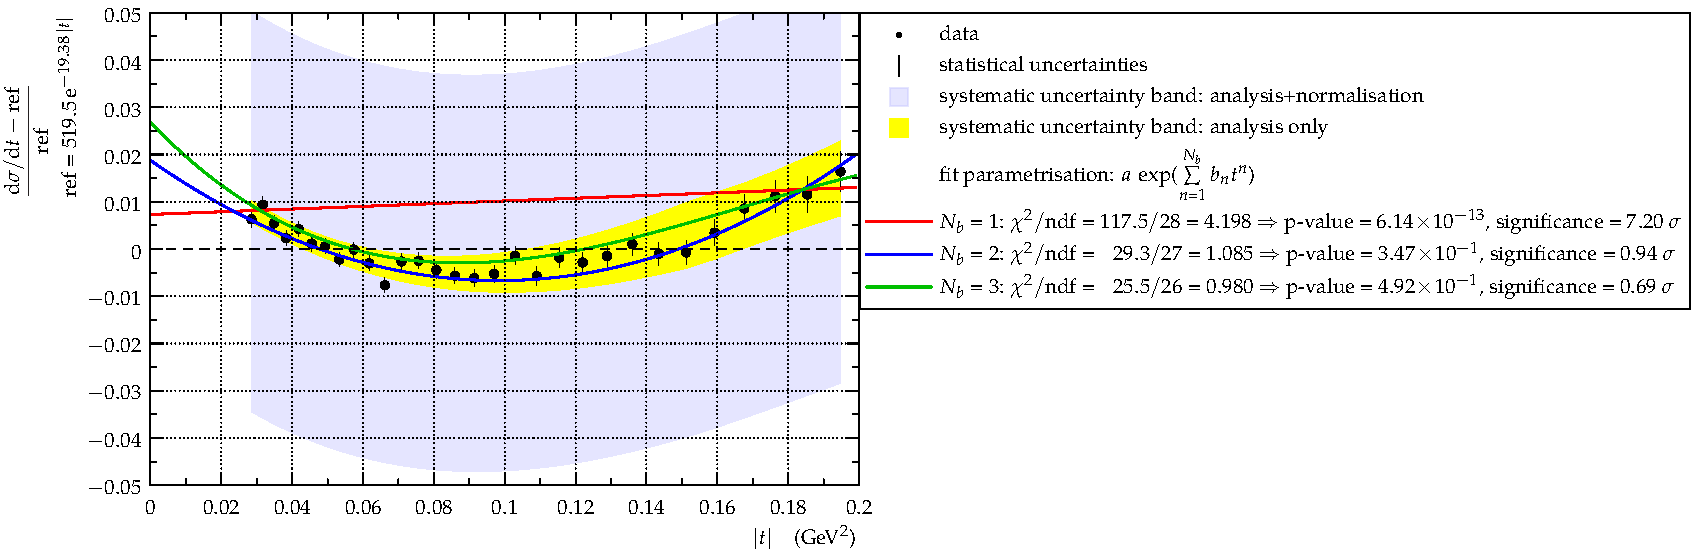
\includegraphics[width=\textwidth]{fig/t_dist_rel_with_fits.pdf}
\vskip-4mm
\caption{%
Differential cross-section using the optimised binning and plotted as relative difference from a reference exponential (see vertical axis). The black dots represent data points with statistical uncertainty bars. The blue band corresponds to the full systematic uncertainty, the yellow one includes all systematic contributions except the normalisation. The coloured lines correspond to fits with parametrisation Eq.~(\ref{fit param}). The red line lies seemingly too high with respect to the data points, which is a consequence of the systematic degrees of freedom included in the fit.
%
Various fit-quality measures are given in the legend, starting with the $\chi^2$ value after minimisation divided by the number of degrees of freedom (ndf). P-value: probability that a $\chi^2$ value greater than the observed one would be drawn from the $\chi^2$ distribution with the given number of degrees of freedom. Significance: half-width of a central region that needs to be excluded from a normal distribution to get the same integrated probability as the p-value.
}
\label{fig:data rel ob}
\end{center}
\vskip-2mm
\end{figure*}



\begin{figure*}
\begin{center}
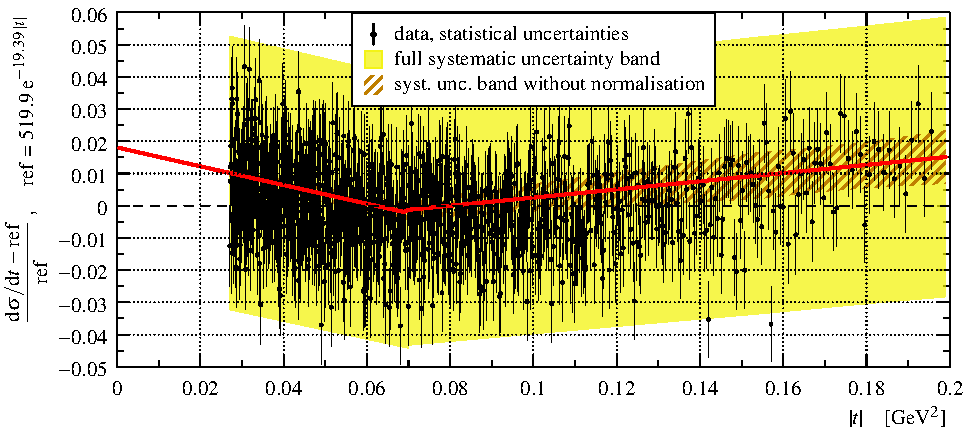
\includegraphics[width=\textwidth]{fig/t_dist_rel_with_split_fit.pdf}
\vskip-4mm
\caption{%
Differential cross-section using the per-mille binning and plotted as relative difference from the reference exponential (see vertical axis). The black dots represent data points with statistical uncertainty bars. The blue band corresponds to the full systematic uncertainty, the yellow one includes all systematic contributions except the normalisation. The green line shows pure exponential fits in regions below and above $|t| = 0.07\un{GeV^2}$.
}
\label{fig:data rel cpb0.001}
\end{center}
\end{figure*}



